\documentclass[letterpaper]{article}
\usepackage{aaai}
\usepackage{times}
\usepackage{helvet}
\usepackage{courier}
\usepackage{algpseudocode}
\usepackage[ruled]{algorithm}
\usepackage{url}
\usepackage{framed}
\usepackage{amsfonts,amsmath,amsthm,amssymb}
\usepackage{graphicx}
\usepackage{url}
\usepackage{color}

\newtheorem{lemma}{Lemma}
\frenchspacing
\pdfinfo{
/Title (MCTS Based on Simple Regret)
/Subject (AAAI Publications)
/Author (AAAI Press)}

\setcounter{secnumdepth}{0}  
\newcommand {\mean} {\ensuremath {\mathop{\mathrm{mean}}}}
\newcommand {\median} {\ensuremath {\mathop{\mathrm{median}}}}
\newcommand {\N} {\ensuremath {\mathcal{N}}}
\newcommand {\IE} {\ensuremath {\mathbb{E}}}
\newcommand {\cov} {\ensuremath {\mathop{\mathrm{cov}}}}
\newcommand {\BEL} {\ensuremath {\mathop{\mathrm{BEL}}}}

\newtheorem{dfn}{Definition}
\newtheorem{thm}{Theorem}
\newtheorem{lmm}{Lemma}
\newtheorem{crl}{Corollary}

\title{MCTS Based on Simple Regret}
\author {David Tolpin, Solomon Eyal Shimony \\
Department of Computer Science, Ben-Gurion University of the Negev, Israel \\
\{tolpin,shimony\}@cs.bgu.ac.il}

\title{MCTS Based on Simple Regret}

\begin{document}

\maketitle

\begin{abstract}
UCT, a state-of-the art algorithm for Monte Carlo tree search (MCTS),
is based on UCB, a policy for the Multi-armed Bandit problem (MAB) that 
minimizes the cumulative regret.  However, search differs from MAB in
that in MCTS it is usually only the final ``arm pull''
that collects a reward, rather than all ``arm pulls''.
Therefore, it makes more sense to minimize the simple, rather than
cumulative, regret. We  introduce policies for
multi-armed bandits with lower simple
regret than UCB and develop a two-stage scheme (SR+CR) for MCTS
which outperforms UCT empirically. In addition, we propose a sampling
scheme based on value of information (VOI), achieving an algorithm
that empirically outperforms other proposed algorithms.
\end{abstract}

\section{Introduction}

Monte-Carlo tree search, and especially a version based on the
UCT formula \cite{Kocsis.uct} appears in numerous search applications,
such as \cite{GellyWang.mogo,Eyerich.ctp}. Although these methods are shown to be successful empirically,
most authors appear to be using the UCT formula ``because it has been shown
to be successful in the past'', and ``because it does a good job of
trading off exploration and exploitation''. While the latter statement may be
correct for the multi-armed bandit and for the UCB method \cite{Auer.ucb},
we argue that it is inappropriate for search. The problem is not that
UCT does not work; rather, a simple reconsideration from basic
principles can result in schemes that outperform UCT.

The core issue is that in adversarial search
and search in ``games against nature'' --- optimizing behavior under
uncertainty, the goal is typically to either find a good (or optimal)
strategy, or even just to find the best first action of such a
policy. Finding a good first action is closer to the pure
exploration variant, as seen in the selection problem
\cite{Bubeck.pure,TolpinShimony.blinkered}. In the selection problem,
it is much better to minimize the \emph{simple} regret.  However, the
simple and the cumulative regret cannot be minimized simultaneously;
moreover, \cite{Bubeck.pure} shows that in many cases the smaller the
cumulative regret, the greater the simple regret.

\section{Background and Related Work}
\label{sec:related-work}

In the {\bf Multi-armed Bandit problem} \cite{Vermorel.bandits} we have a set
of $K$ arms. Each arm can
be pulled multiple times. Sometimes a cost is
associated with each pulling action. When the $i$th arm
is pulled, a random reward $X_i$ from an unknown stationary
distribution is encountered.
In the cumulative setting (the focus of much of the research literature on Multi-armed bandits),
all encountered rewards are collected by the agent. 
The UCB scheme was shown to be near-optimal in this respect \cite{Auer.ucb}:

\begin{dfn} Scheme $\mathbf{UCB(c)}$ pulls arm $i$ that maximizes 
upper confidence bound $b_i$ on the reward:
\begin{equation}
b_i=\overline X_i+\sqrt {{c \log (n)} / {n_i}}
\label{eqn:ucb}
\end{equation}
where $\overline X_i$ is the average sample reward obtained from arm $i$,
$n_i$ is the number of times arm $i$ was pulled, and $n$ is the total
number of pulls so far. \end{dfn} 

The {\bf UCT algorithm,} an extension of UCB
to Monte-Carlo Tree Search is described in \cite{Kocsis.uct}, and
shown to outperform many state of the art search algorithms in both
MDP and adversarial games \cite{Eyerich.ctp,GellyWang.mogo}. 

In the {\bf simple regret (selection) setting}, the agent gets to
collect only the reward of the last pull. An upper bound on the simple
regret of uniform sampling is exponentially decreasing in the number
of samples (see \cite{Bubeck.pure}, Proposition~1). For UCB($c$) the
best known respective upper bound on the simple regret of UCB($c$) is
only polynomially decreasing in the number of samples (see
\cite{Bubeck.pure}, Theorems~2,3). However, empirically UCB($c$)
appears to yield a lower simple regret than uniform sampling.

A completely different scheme for control of sampling can use the
principles of {\bf bounded rationality} \cite{Horvitz.reasoningabout}
and {\bf rational metareasoning} \cite{Russell.right}. In search, one
maintains a current best move $\alpha $ at the root, and finds the
expected gain from finding another move $\beta $ to be better than the
current best. We introduce in this paper simple
schemes loosely based on the metareasoning concept of value of
information, and compare them to UCB (on sets) and UCT (in trees).


\section{Sampling Based on Simple Regret}
\label{sec:results}

\subsection{Analysis of Sampling on Sets}
\label{sec:sampling-on-sets}


We examine some sampling schemes with super-polynomially
decreasing upper bounds on the simple regret. The bounds
suggest that these schemes achieve a lower simple regret
than uniform sampling; indeed, this is confirmed
by experiments. First, we consider $\varepsilon$-greedy sampling as a straightforward
generalization of uniform sampling:
\begin{dfn} The \textbf{$\mathbf{\varepsilon}$-greedy} sampling scheme
pulls the arm that currently has the greatst sample mean, with probability
$0<\varepsilon<1$, and any other
arm with probability $\frac {1-\varepsilon} {K-1}$. 
\end{dfn}
This sampling scheme exhibits an exponentially decreasing simple
regret.
In particular, as the number of arms $K$ grows, the bound for $\frac 1
2$-greedy sampling ($\varepsilon=\frac 1 2$) becomes considerably tighter than for uniform
random sampling ($\varepsilon=\frac 1 K$):
\begin{thm}
For uniform random sampling, 
\begin{equation}
\IE r_{uniform}\le 2\gamma \sum_{i=1}^K\Delta_i\exp\left(-\frac {\Delta_i^2n} {K}\right)
\end{equation}
For $\frac 1 2$-greedy sampling,
\begin{eqnarray}
\IE r_{\frac 1 2\mbox{-}greedy}&\le& 2\gamma \sum_{i=1}^K\Delta_i\exp\left(\frac {-2\Delta_i^2n}
  {\left(1+\sqrt{K-1}\right)^2}\right)
\end{eqnarray}
\end{thm}

Another sampling scheme for simple regret minimization can be obtained
by distributing samples in a way similar to UCB, but sampling the current best arm
less often. This can be achieved by replacing $\log(\cdot)$ in
Equation~\ref{eqn:ucb} with a faster growing function, e.g. $\sqrt\cdot$.
\begin{dfn} Scheme $\mathbf{UCB_{\sqrt{\cdot}}(c)}$ pulls arm $i$ that
maximizes $b_i$, where $b_i=\overline X_i+\sqrt {{c \sqrt n} / {n_i}}$.
\end{dfn}
This scheme also exhibits a super-polynomially decreasing simple regret.

\subsection{Sampling in Trees}
\label{sec:sampling-in-trees}

As mentioned above, UCT \cite{Kocsis.uct} is an extension of UCB for
MCTS, that applies UCB($c$) at each step of a rollout.  At the root
node, the sampling in MCTS is usually aimed at finding the first move
to perform. Search is re-started, either from scratch or using some
previously collected information, after observing the actual outcome
(in MDPs) or the opponent's move (in adversarial games). Once one move
is shown to be the best choice with high confidence, the value of
information of additional samples of the best move (or, in fact, of
any other samples) is low. Therefore, one should be able to do better
than UCT by optimizing {\em simple regret}, rather than {\em
cumulative regret}, at the root node.

However, for thee internal nodes optimizing simple regret is not the
answer, and cumulative regret optimization is not so far off the
mark. Our suggested improvement to UCT is the \textbf{SR+CR MCTS
sampling scheme} that combines different sampling schemes on the first
step and during the rest of each rollout.  We expect such two-stage
sampling schemes to outperform UCT and be significantly less sensitive
to the tuning of the exploration factor $c$ of UCB($c$).


\subsection{VOI-aware Sampling}
\label{sec:voi-sampling}

Further improvement can be achieved by computing or estimating the
value of information (VOI) of the rollouts and choosing rollouts that
maximize the VOI. We estimate the VOI from
the current set of samples:
\begin{eqnarray}
VOI_\alpha&\approx&\frac {\overline X_\beta} {n_\alpha+1}
\exp\left(-2(\overline X_\alpha - \overline X_\beta)^2 n_\alpha\right)\\
VOI_i&\approx&\frac {1-\overline X_\alpha} {n_i+1}
\exp\left(-2(\overline X_\alpha - \overline X_i)^2 n_i\right),\; i\ne\alpha\nonumber\\
\mbox{where }&&\alpha=\arg\max_i \overline X_i,\quad
             \beta=\arg\max_{i,\,i\ne\alpha} \overline X_i\nonumber
\end{eqnarray}
The ``VOI-aware'' scheme samples the action that has the maximum
estimated VOI.  Although this scheme appears too complicated for
a formal analysis, early experiments demonstrate a significantly lower
simple regret.


\section{Empirical Evaluation}
\label{sec:emp}

The results were empirically verified on Multi-armed Bandit instances,
on search trees, and on the sailing domain, as defined in
\cite{Kocsis.uct}. In most cases, the experiments showed a lower average
simple regret for $\frac 1 2$-greedy an UCB$_{\sqrt{\cdot}}$ than for
UCB on sets, and for the SR+CR scheme than for UCT in trees.

Figure~\ref{fig:mcts-regret} shows
results for experiments on randomly generated trees. VOI+UCT, the scheme based on a VOI estimate,
outperforms all other sampling schemes in this example; either $\frac 1
2$-greedy+UCT or UCB$_{\sqrt{\cdot}}$+UCT
result in the second lowest regret, UCB$_{\sqrt{\cdot}}$+UCT dominates UCT everywhere
except when the number of samples is small. The advantage of both $\frac 1
2$-greedy+UCT and UCB$_{\sqrt{\cdot}}$+UCT grows with the number of arms.
\begin{figure}[h!]
  \centering
  \includegraphics[scale=0.5]{tree-identity-k=32-uqb=8+voi.pdf}\\
  \caption{MCTS in random trees.}
  \label{fig:mcts-regret} 
\end{figure}

Figure~\ref{fig:sailing-cost-vs-nsamples}
shows results of experiments on the sailing
domain. UCT is always worse than either $\frac 1 2$-greedy+UCT or
UCB$_{\sqrt{\cdot}}$+UCT.

\begin{figure}[h!]
  \centering
  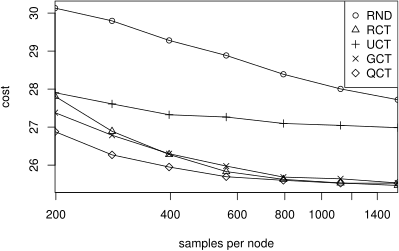
\includegraphics[scale=0.45]{costs-size=6-group=median.pdf}\\
  \caption{The sailing domain, $6\times 6$ lake, cost vs. samples}
  \label{fig:sailing-cost-vs-nsamples}
\end{figure}


\section{Conclusion and Future Work}
\label{sec:summary}

UCT-based Monte-Carlo tree search has been shown to be very effective
for finding good actions in both MDPs and adversarial games.
Further improvement of the sampling scheme is thus of interest in
numerous search applications. We argue that although UCT is already very efficient,
one can do better if the sampling scheme is considered from a metareasoning
perspective of value of information (VOI).

The MCTS SR+CR scheme presented in the paper differs
from UCT mainly in the first step of the rollout, when we attempt to minimize
the `simple' selection regret rather than the cumulative regret. Both the
theoretical analysis and the empirical evaluation provide evidence for
better general performance of the proposed scheme.

Although SR+CR is inspired by the notion of VOI,
the VOI is used there implicitly in the analysis of the algorithm,
rather than computed or learned explicitly in order to plan the
rollouts. Ideally, using VOI to control sampling ab-initio should do even better,
but the theory for doing that is still not up to speed. Instead we suggest
a  ``VOI-aware'' sampling scheme based on crude probability and value estimates,
which despite its simplicity already shows a marked improvement in minimizing regret.
However, application of the theory of rational metareasoning
to Monte Carlo Tree Search is an open problem \cite{HayRussell.MCTS},
and both a solid theoretical model and empirically efficient VOI
estimates need to be developed. 

Finding a better sampling scheme for non-root nodes,
as well as the root node, should also be possible.
Although cumulative regret does reasonably
well there, it is far from optimal, as meta-reasoning principles imply that an optimal scheme
for these nodes must be asymmetrical (e.g. it is not helpful to find out that the
value of the current best action is even better than previously believed).

Finally, applying VOI methods in complex deployed applications that already use
MCTS is a challenge that should be addressed in future work.
In particular, UCT is extremely successful in Computer
Go \cite{GellyWang.mogo,Braudis.pachi,Enzenberger.Fuego},
and the proposed scheme should be evaluated on this domain. This is non-trivial, since
Go programs typically use ``non-pure'' versions of UCT, extended with
domain-specific knowledge. For example, Pachi \cite{Braudis.pachi}
typically re-uses information from rollouts generated for earlier
moves, thereby violating our underlying assumption that information is
only used for selecting the current move.  In early experiments not
shown here (disallowing re-use of samples, admittedly not really a
fair comparison) the VOI-aware scheme apears to dominate UCT.
Nevertheless, it should also be possible to adapt the VOI-aware
schemes to take into account expected re-use of samples, another topic
for future research.


\section*{Acknowledgments}

The research is partially supported by Israel
Science Foundation grant 305/09, by the Lynne and William Frankel
Center for Computer Sciences, and by the Paul Ivanier Center for
Robotics Research and Production Management.

\bibliographystyle{aaai}
\bibliography{refs}


\end{document}
